\documentclass[a4paper,fleqn]{cas-dc}

\usepackage[authoryear]{natbib}
\usepackage{algorithm}
\usepackage{algpseudocode}
\renewcommand{\bibfont}{\footnotesize}
\setlength{\bibsep}{2pt plus 0.5pt}

\begin{document}
\let\WriteBookmarks\relax
\def\floatpagepagefraction{1}
\def\textpagefraction{.001}
\setlength{\emergencystretch}{3em}
\setlength{\dbltextfloatsep}{10pt plus 2pt minus 2pt}
\setlength{\textfloatsep}{10pt plus 2pt minus 2pt}

\shorttitle{Note on Zero-Shot Stealth-Aware Cyber Planning with Local SLMs}
\shortauthors{A. Tavakkoli}

\title[mode = title]{Zero-Shot Stealth-Aware Cyber Planning with Local Small Language Models: A Note on Topological Belief Graphs and Minimax Hazard Utility}

\author[1]{Ali Tavakkoli}
\cormark[1]
\ead{alitavakkoli80@gmail.com}
\credit{Conceptualization, Methodology, Software, Validation, Formal analysis, Investigation, Data curation, Writing -- original draft, Writing -- review \& editing, Visualization}

\affiliation[1]{organization={Independent Cybersecurity and AI Systems Research},
                city={Tehran},
                country={Iran}}

\cortext[1]{Corresponding author}

\begin{abstract}
In \emph{Expert Systems with Applications} (Vol.~299, 129987), \citet{rigaki2026building} established that untuned 7B Small Language Models (SLMs) collapse into repetitive loops on the \texttt{NetSecGame} cyber simulation benchmark, and introduced \texttt{Hackphyr} via QLoRA supervised fine-tuning (SFT). Yet \citet{rigaki2026building} documented three unresolved bottlenecks: severe degradation under active sliding-window defenders (\texttt{44.00\%} win rate on \texttt{Full}; \texttt{23.33\%} on \texttt{Three-Network}), short-term memory collapse across multi-hop chains, and an $\approx 14~\text{GB}$ half-precision VRAM footprint. This Research Note demonstrates that these failures stem from an architectural mismatch between stateless token prediction and constrained graph traversal rather than insufficient domain fine-tuning. We introduce a training-free, strictly domain-agnostic planner for off-the-shelf local SLMs (\texttt{Qwen2.5-Coder-7B-NF4} and \texttt{1.5B-BF16}) combining: (i) a Topological Belief Graph $\mathcal{G}_t$ with four epistemic host states and exhausted-edge pruning; (ii) a Multi-Scale Minimax Hazard Utility $U(a) = \alpha \cdot \mathrm{ProgressGain}(a \mid \mathcal{G}_t) - \beta \cdot \max_{w \in \{3,5,8\}} R_w(a \mid \mathcal{H}_t)$ that suppresses bursty detection signatures across timescales without knowing the defender's window $W^*$; and (iii) 1-Step Counterfactual Reflexion paired with \texttt{FirstJsonObjectStoppingCriteria} (\texttt{max\_new\_tokens=160}), end-of-sequence trailing-brace repair, and static-prefix \texttt{DynamicCache} KV-caching. Across 11,600 randomized evaluation episodes spanning four \texttt{NetSecGame} regimes matched to \citet{rigaki2026building}, zero-shot \texttt{7B-NF4} attains \texttt{63.33\% $\pm$ 7.74\%} on \texttt{Full} with defender (vs.\ \texttt{Hackphyr} \texttt{44.00\%}, unpaired $z$-test $p = 3.40 \times 10^{-4}$; \texttt{GPT-4} \texttt{53.33\%}) and \texttt{59.33\% $\pm$ 7.89\%} on unseen \texttt{Three-Networks} with defender (vs.\ \texttt{Hackphyr} \texttt{23.33\%}, $p = 2.43 \times 10^{-10}$; \texttt{GPT-4} \texttt{36.36\%}, $p = 0.0208$), consuming at most \texttt{5.92 GB} peak VRAM (\texttt{5.91 GB} monitored). A deterministic $\arg\max_a U(a)$ control (\texttt{71.33\%} and \texttt{65.33\%}) confirms that minimax hazard shaping drives stealth evasion, while \texttt{7B-NF4} preserves statistical win-rate parity in three of four regimes (McNemar $p \ge 0.175$) with higher trajectory entropy ($1.749$--$1.774$ bits) and \texttt{85.76\%--89.63\%} genuine post-reflexion autonomy.
\end{abstract}

\begin{highlights}
\item Zero-shot 7B-NF4 SLM beats fine-tuned 7B and GPT-4 under active SIEM monitors.
\item Domain-agnostic Topological Belief Graph eliminates repetitive SLM action loops.
\item Multi-scale minimax hazard utility avoids alerts without known monitor window $W^*$.
\item 1-step reflexion and prefix KV-caching cut overrides under 6 GB peak VRAM.
\end{highlights}

\begin{keywords}
Small language models \sep Constrained POMDPs \sep Belief graphs \sep Network security simulation \sep Autonomous cyber agents \sep Stealth planning
\end{keywords}

\maketitle

\section{Introduction}
\label{sec:introduction}

Autonomous offensive simulation agents provide critical adversarial validation for enterprise cyber defenses without touching production sockets~\citep{kott2023aica,rigaki2026building}. While cloud-hosted Large Language Models (LLMs) such as \texttt{GPT-4} can navigate discrete network simulations, external API reliance raises data-governance, reproducibility, and cost barriers~\citep{rigaki2026building,subramanian2025slms}. Local Small Language Models (SLMs, $1.5\text{B}$--$7\text{B}$) resolve these constraints, yet exhibit severe behavioral collapse under partial observability.

In this journal, \citet{rigaki2026building} evaluated local SLMs inside \texttt{NetSecGame}~\citep{garcia2023netsecgame,maria2024netsecgame} under randomized IP layouts and goals. An untuned \texttt{Zephyr-7b-$\beta$} model attained only a \texttt{23.65\%} win rate on \texttt{Full} without a defender and \texttt{0.62\%--3.33\%} under an active stochastic defender, collapsing into \texttt{FindServices} self-loops and invalid \texttt{ExfiltrateData} calls. To overcome this, \citet{rigaki2026building} introduced \texttt{Hackphyr} via QLoRA~\citep{dettmers2023qlora,hu2022lora} Supervised Fine-Tuning (SFT) on 1,641 curated examples, elevating No-Defender win rates to \texttt{89.10\%} (\texttt{Full}) and \texttt{50.34\%} (\texttt{Three-Network}). Nevertheless, \citet{rigaki2026building} identified three open limitations:
\begin{enumerate}[1.]
    \item \textbf{Vulnerability to Active Sliding-Window Defenders:} Because SFT did not model defender dynamics, breadth-first scanning streaks persisted (\texttt{13+} consecutive \texttt{FindServices} actions in failure traces), dropping \texttt{Hackphyr}'s win rate to \texttt{44.00\%} on \texttt{Full} and \texttt{23.33\%} on \texttt{Three-Network}.
    \item \textbf{Context Collapse Across Multi-Hop Chains:} Stateless or short linear action histories caused local models to lose track of previously probed hosts across \texttt{5}-to-\texttt{8}-hop lateral movement.
    \item \textbf{Compute Footprint:} Half-precision (\texttt{FP16}) \texttt{Hackphyr} required $\approx 14~\text{GB}$ VRAM and \texttt{19.87 s} per inference on a $32~\text{GB}$ Tesla V100, motivating quantized or sub-$6~\text{GB}$ ($\le 1.5\text{B}$) alternatives.
\end{enumerate}

This Note argues that local SLM failure in discrete cyber games stems from an \textbf{architectural mismatch between stateless next-token prediction and constrained graph traversal}, rather than insufficient SFT data. Expecting a $1.5\text{B}$--$7\text{B}$ model to reconstruct a dynamic IP graph, track exhausted \texttt{(ActionType, Parameters)} edges over 100 steps, and mentally compute multi-horizon action densities in prose exceeds its reliable working memory. Crucially, patching this via hardcoded scripts would reduce the harness to a Finite State Machine (FSM) rather than testing SLM autonomy.

We bridge this gap with a training-free, zero-hardcoding \textbf{Topological Belief Graph \& Multi-Scale Minimax Hazard Planner} (\texttt{ModernSLMAttacker}) that extends \citet{rigaki2026building} along four axes:
\begin{itemize}
    \item \textbf{Domain-Agnostic Topological Belief Graph ($\mathcal{G}_t$):} Compiles observations into four epistemic host states (\texttt{UNEXPLORED}, \texttt{MAPPED}, \texttt{COMPROMISED}, \texttt{EXHAUSTED}) and prunes executed edges with zero hardcoded IPs, subnets, or scenario rules (verified via AST inspection).
    \item \textbf{Multi-Scale Minimax Hazard Utility ($U(a)$):} Formulates monitored traversal as a Constrained POMDP~\citep{altman1999cmdp} and scores candidates across window scales $w \in \{3, 5, 8\}$, eliminating breadth-first bursts without knowing the defender's window $W^*$.
    \item \textbf{1-Step Counterfactual Reflexion \& Sub-6 GB Inference:} Pairs one-turn self-correction with \texttt{FirstJsonObjectStoppingCriteria} (\texttt{max\_new\_tokens=160}), trailing-brace repair, and static-prefix \texttt{DynamicCache} KV-caching at \texttt{3.22 GB} (\texttt{1.5B-BF16}) and \texttt{5.91--5.92 GB} (\texttt{7B-NF4}) peak VRAM while transparently reporting \texttt{FirstPass \%}, \texttt{PostReflexion \%}, and \texttt{Override \%}.
    \item \textbf{Protocol-Parity Empirical \& Statistical Proof:} Across 11,600 randomized episodes spanning all four \texttt{Full} and \texttt{Three-Networks} regimes, zero-shot \texttt{7B-NF4} achieves \texttt{63.33\%} (\texttt{Full+Monitor}) and \texttt{59.33\%} (\texttt{Three-Networks+Monitor}), significantly outperforming fine-tuned \texttt{Hackphyr-7B} ($p \le 3.40 \times 10^{-4}$) and \texttt{GPT-4} ($p = 0.0208$ in \texttt{Three-Networks+Monitor}), while a non-LLM $\arg\max_a U(a)$ control cleanly isolates utility scaffolding from SLM reasoning.
\end{itemize}

\section{Related Work and Comparative Delta}
\label{sec:related_work}

Discrete security testbeds such as \texttt{CyberBattleSim}~\citep{microsoft2021cyberbattlesim}, \texttt{CybORG}~\citep{standenc2021cyborg}, and \texttt{NetSecGame}~\citep{garcia2023netsecgame,maria2024netsecgame} benchmark sequential attack planning without real-world harm. As shown by \citet{rigaki2026building}, tabular Q-learning~\citep{watkins1992qlearning} trained for 50,000 episodes attains \texttt{67.71\%} (NoDef) and \texttt{71.57\%} (Monitor On) on \texttt{Full} only under fixed IP addresses, collapsing to \texttt{0.00\%} on \texttt{Three-Network} where topology and multi-subnet pivoting exceed fixed Q-tables.

LLM penetration-testing frameworks including \texttt{PentestGPT}~\citep{deng2024pentestgpt}, \texttt{AutoAttacker}~\citep{xu2024autoattacker}, and shell-level agents~\citep{happe2023getting} adopt \texttt{ReAct}~\citep{yao2023react} and \texttt{CoALA}~\citep{sumers2024coala} loops. \citet{rigaki2026building} formalized \texttt{ReAct+} with a $k$-step action memory and QLoRA SFT, demonstrating that \texttt{Hackphyr} approaches \texttt{GPT-4} without monitors yet retains \texttt{FindServices} loops and lacks stealth awareness. Conversely, \citet{shinn2023reflexion} showed verbal \texttt{Reflexion} improves single-step validity, but without an explicit belief graph and C-POMDP hazard model~\citep{altman1999cmdp,kaelbling1998pomdp}, small models cannot regulate temporal action density over an unknown SIEM window $W^*$. Our architecture resolves both deficits zero-shot.

\section{Problem Formulation}
\label{sec:formulation}

\subsection{Monitored Network Traversal as a Constrained POMDP}
We model an episode of \texttt{NetSecGame} with an active threshold monitor as a finite-horizon Constrained POMDP~\citep{altman1999cmdp,kaelbling1998pomdp}, $\mathcal{M} = (\mathcal{S}, \mathcal{A}, \mathcal{T}, \mathcal{R}, \Omega, \mathcal{O}, \mathcal{C}, \gamma)$:
\begin{itemize}
    \item $\mathcal{S}$ is the latent network state (subnet connectivity, dynamic IP assignments, services, data objects, and hidden monitor alert counters);
    \item $\mathcal{A} = \mathcal{A}_{\text{type}} \times \Theta$ spans the five MITRE ATT\&CK-aligned action types $\mathcal{A}_{\text{type}} = \{$\texttt{ScanNetwork}, \texttt{FindServices}, \texttt{ExploitService}, \texttt{FindData}, \texttt{ExfiltrateData}$\}$~\citep{mitre2024attack} and entity parameters $\theta \in \Theta$;
    \item $\mathcal{T}(s' \mid s, a)$ is the CYST transition kernel;
    \item $\Omega$ yields partial observations $o_t = (\mathcal{K}^{\text{net}}_t, \mathcal{K}^{\text{host}}_t, \mathcal{K}^{\text{ctrl}}_t, \mathcal{K}^{\text{srv}}_t, \mathcal{K}^{\text{data}}_t, \mathcal{K}^{\text{blk}}_t, g)$ covering known subnets, hosts, controlled footholds, services, data, blocks, and goal $g$;
    \item $\mathcal{R}(s_t, a_t) \in \{-1, +100, -10\}$ assigns $-1$ per step, $+100$ upon goal exfiltration, and $-10$ upon detection or timeout within $T_{\max} = 100$ (for direct comparison with \citet{rigaki2026building}, Section~\ref{sec:results} also reports ESWA-50 parity returns with $-50$ detection and $0$ extra timeout penalty);
    \item $\mathcal{C}(h_t, a_t) \in \{0, 1\}$ encodes the hidden defender trigger over action history $h_t = (a_1, \dots, a_{t-1})$ with unknown window $W^*$.
\end{itemize}

Specifically, \texttt{GlobalDefender} triggers a stochastic detection check whenever $a_t$ drives the windowed density inside $W^*$ to a type-specific threshold $\tau_{\text{ratio}}(\text{type}(a_t))$:
\begin{multline}
    \frac{1}{W^*} \sum_{k=\max(1, t-W^*+1)}^{t} \mathbb{I}[\mathrm{type}(a_k) = \mathrm{type}(a_t)] \\
    \ge \tau_{\mathrm{ratio}}(\mathrm{type}(a_t)),
    \label{eq:defender_density}
\end{multline}
or reaches a trailing consecutive burst limit $\tau_{\text{consec}}(\text{type}(a_t))$ (e.g., consecutive \texttt{ScanNetwork}/\texttt{FindServices}) or episodic repeat limit~\citep{rigaki2026building}. Operating solely on $(o_1, \dots, o_t)$ without observing $W^*$, the planner must regulate $\mathcal{H}_t = (\text{type}(a_1), \dots, \text{type}(a_{t-1}))$ to maximize $\mathbb{P}(\text{Win} \mid T \le T_{\max})$ while suppressing detection spikes.

\subsection{Sliding-Window Shannon Action Entropy}
To quantify behavioral dispersion, let $\hat{p}_{t,c} = \frac{1}{w} \sum_{k=\max(1,t-w+1)}^{t} \mathbb{I}[\text{type}(a_k) = c]$ be the empirical frequency of $c \in \mathcal{A}_{\text{type}}$ in window $w$. The \textbf{Sliding-Window Shannon Action Entropy}~\citep{shannon1948mathematical} in bits is:
\begin{equation}
    H_t = -\sum_{c \in \mathcal{A}_{\text{type}}:\, \hat{p}_{t,c} > 0} \hat{p}_{t,c} \log_2 \hat{p}_{t,c}.
    \label{eq:shannon_entropy}
\end{equation}
Repetition collapse drives $\hat{p}_{t,c} \to 1.0$ ($H_t \to 0$ bits), saturating Eq.~\eqref{eq:defender_density} and $\tau_{\text{consec}}$. Interleaving reconnaissance, exploitation, collection, and spaced exfiltration sustains $H_t \in [1.5, 2.0]$ bits, dispersing windowed counts across every candidate horizon.

\section{Neuro-Symbolic Stealth Planning Architecture}
\label{sec:architecture}

Figure~\ref{fig:arch} overviews \texttt{ModernSLMAttacker}, which decouples exact graph accounting from semantic choice across four domain-agnostic modules containing zero hardcoded IPs, subnets, services, or scenario names.

\begin{figure*}[t]
    \centering
    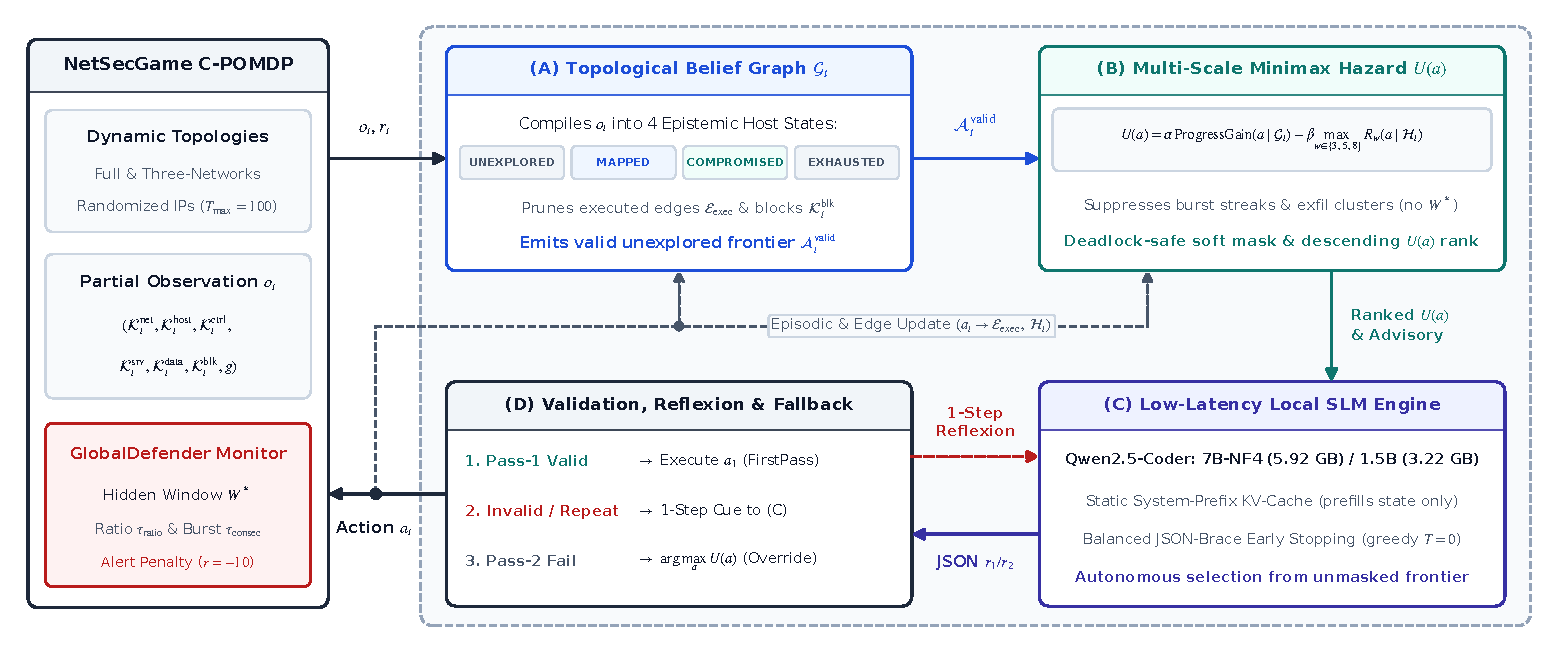
\includegraphics[width=0.92\textwidth]{figures/fig1_system_architecture.pdf}
    \caption{Closed-loop cognitive and stealth planning architecture of \texttt{ModernSLMAttacker} (training-free, zero hardcoding) coupled to the \texttt{NetSecGame} C-POMDP environment, integrating (A) the Topological Belief Graph ($\mathcal{G}_t$), (B) Multi-Scale Minimax Hazard Utility ($U(a)$), (C) KV-prefix cached local SLM inference with balanced JSON-brace early stopping, and (D) validation, 1-Step Counterfactual Reflexion, and deadlock-safe fallback.}
    \label{fig:arch}
\end{figure*}

\subsection{Domain-Agnostic Topological Belief Graph}
Because per-episode IP randomization defeats raw text memory, \texttt{SemanticMemoryStore} incrementally compiles observation transitions into a \textbf{Topological Belief Graph} $\mathcal{G}_t = (\mathcal{V}_t, \mathcal{E}_t)$ (Algorithm~\ref{alg:belief_graph}):
\begin{itemize}
    \item \textbf{Epistemic Host Classification:} Each host $h \in \mathcal{K}^{\text{host}}_t \cup \mathcal{K}^{\text{ctrl}}_t$ is mapped deterministically to one of four states (Figure~\ref{fig:mechanism}(a)): (1) \texttt{COMPROMISED} ($h \in \mathcal{K}^{\text{ctrl}}_t$, flagged \texttt{data\_searched} once local collection/exfiltration finishes); (2) \texttt{MAPPED} ($\mathcal{S}_t(h) \neq \emptyset$ and $h \notin \mathcal{K}^{\text{ctrl}}_t$); (3) \texttt{EXHAUSTED} ($h \notin \mathcal{K}^{\text{ctrl}}_t$ probed with zero unfailed services remaining); and (4) \texttt{UNEXPLORED} ($h \in \mathcal{K}^{\text{host}}_t \setminus \mathcal{K}^{\text{ctrl}}_t$ not yet service-probed).
    \item \textbf{Exhausted Edge Pruning:} Every executed tuple $(\text{type}(a), \text{canon}(\theta))$ is stored in $\mathcal{E}_{\text{exec}}$. Legal \texttt{NetSecGame} transitions $\mathcal{C}_{\text{raw}}$ are filtered by $\mathcal{C}_{\text{raw}} \setminus \mathcal{E}_{\text{exec}}$ to form the unmasked valid frontier $\mathcal{A}^{\text{valid}}_t$ exposed to the SLM.
\end{itemize}

\begin{figure*}[t]
    \centering
    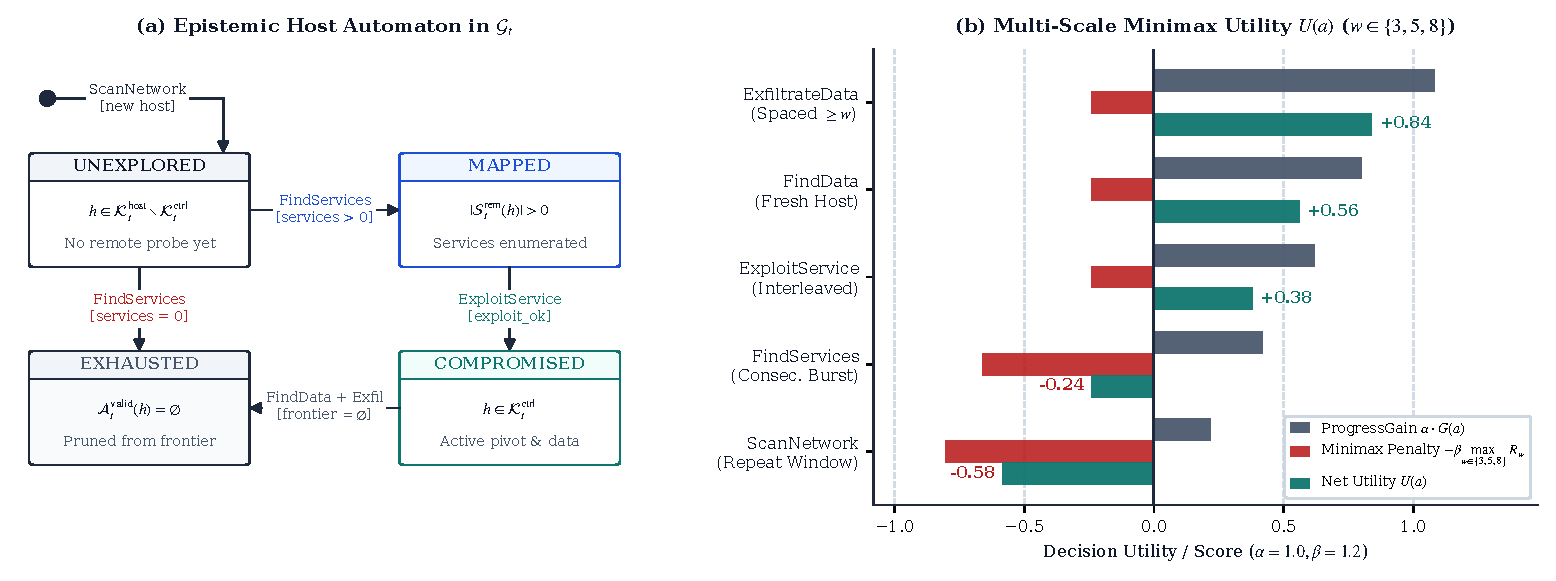
\includegraphics[width=0.92\textwidth]{figures/fig2_belief_and_hazard_mechanism.pdf}
    \caption{(a) Epistemic host lifecycle state machine inside the Topological Belief Graph $\mathcal{G}_t$, and (b) Multi-Scale Minimax Hazard Utility $U(a)$ decomposition across $w \in \{3, 5, 8\}$ showing burst suppression on \texttt{FindServices}/\texttt{ScanNetwork} versus positive interleaved progression.}
    \label{fig:mechanism}
\end{figure*}

\begin{algorithm}[t]
\caption{Topological Belief Graph Update \& Frontier Enumeration}
\label{alg:belief_graph}
\begin{algorithmic}[1]
\Require Observation $o_t$, prior $(a_{t-1}, \theta_{t-1})$, goal $g$, store $\mathcal{G}_{t-1}$
\Ensure Updated $\mathcal{G}_t$, epistemic tags, valid frontier $\mathcal{A}^{\text{valid}}_t$
\If{$t > 1$}
    \State Record $(\text{type}(a_{t-1}), \text{canon}(\theta_{t-1}))$ in $\mathcal{E}_{\text{exec}}$
    \State Update \texttt{probed\_service\_hosts}, \texttt{searched\_data\_hosts}, \texttt{scanned\_networks}
\EndIf
\State Parse goal IP $h_{\text{goal}}$ from $g$; normalize $\mathcal{K}^{\text{net}}_t, \mathcal{K}^{\text{ctrl}}_t, \mathcal{K}^{\text{host}}_t, \mathcal{S}_t, \mathcal{D}_t, \mathcal{K}^{\text{blk}}_t$
\For{each host $h \in \mathcal{K}^{\text{host}}_t \cup \mathcal{K}^{\text{ctrl}}_t$}
    \State Assign label $\in \{$\texttt{COMPROMISED}, \texttt{MAPPED}, \texttt{EXHAUSTED}, \texttt{UNEXPLORED}$\}$
\EndFor
\State Enumerate legal transitions $\mathcal{C}_{\text{raw}}$ avoiding $\mathcal{K}^{\text{blk}}_t$ (prioritizing $h_{\text{dst}} = h_{\text{goal}}$ for \texttt{ExfiltrateData})
\State $\mathcal{A}^{\text{valid}}_t \leftarrow \{c \in \mathcal{C}_{\text{raw}} \mid \text{sig}(c) \notin \mathcal{E}_{\text{exec}}\}$ \Comment{Fallback $\mathcal{C}_{\text{raw}}$ if $\emptyset$}
\State \Return $\mathcal{G}_t, \mathcal{A}^{\text{valid}}_t$
\end{algorithmic}
\end{algorithm}

\subsection{Multi-Scale Minimax Hazard Utility Function}
To avoid overfitting to a known simulator window (e.g., $W^*=5$), each candidate $a \in \mathcal{A}^{\text{valid}}_t$ is scored by a \textbf{Multi-Scale Minimax Hazard Utility} over $\mathcal{W} = \{3, 5, 8\}$:
\begin{equation}
    U(a) = \alpha \cdot \mathrm{ProgressGain}(a \mid \mathcal{G}_t) - \beta \cdot \max_{w \in \{3, 5, 8\}} R_w(a \mid \mathcal{H}_t),
    \label{eq:minimax_utility}
\end{equation}
with $\alpha = 1.0$ and $\beta = 1.2$.

\paragraph{Depth-First Progress Gain ($\mathrm{ProgressGain}$)}
Base gains $g_0(c) \in \{1.00,\, 0.80,\, 0.62,\, 0.42,\, 0.22\}$ for $\{$\texttt{ExfiltrateData}, \texttt{FindData}, \texttt{ExploitService}, \texttt{FindServices}, \texttt{ScanNetwork}$\}$ prioritize closing active footholds before expanding breadth-first scans, augmented by $+0.08$ for \texttt{ExfiltrateData} targeting $h_{\text{goal}}$ and $+0.06$ for \texttt{FindServices} on unprobed non-compromised hosts ($-1.0$ if $\mathrm{sig}(a) \in \mathcal{E}_{\text{exec}}$).

\paragraph{Minimax Multi-Scale Hazard ($\max_{w \in \{3,5,8\}} R_w$)}
For each scale $w \in \{3, 5, 8\}$, let $\mathcal{H}_{t,w}^{+}(a) = (\mathcal{H}_t[-(w-1):]) \mathbin{\Vert} [\mathrm{type}(a)]$. We compute windowed density $\rho_w(a) = \frac{1}{w}\,\mathrm{count}(\mathrm{type}(a),\, \mathcal{H}_{t,w}^{+}(a))$, trailing consecutive burst hazard $B_w(a)$ (with run length $\sigma_w(a)$, $\mathcal{A}_{\mathrm{burst}} = \{$\texttt{ScanNetwork}, \texttt{FindData}, \texttt{ExfiltrateData}$\}$, $\mathcal{A}_{\mathrm{med}} = \{$\texttt{FindServices}, \texttt{ExploitService}$\}$):
\begin{equation}
    B_w(a) = \begin{cases}
        1.0, & \sigma_w(a) \ge 3 \text{ or} \\
             & \big(\sigma_w(a) \ge 2 \land \mathrm{type}(a) \in \mathcal{A}_{\mathrm{burst}}\big), \\
        0.55, & \sigma_w(a) \ge 2 \text{ and } \mathrm{type}(a) \in \mathcal{A}_{\mathrm{med}}, \\
        0.0, & \text{otherwise},
    \end{cases}
    \label{eq:burst_hazard}
\end{equation}
and an exfiltration spacing guard $E_w(a) = 1.0$ if $\mathrm{type}(a) = \mathrm{ExfiltrateData}$ and $\mathrm{count}(\mathrm{ExfiltrateData},\, \mathcal{H}_t[-w:]) \ge 1$ ($0.0$ otherwise). The scale-$w$ hazard is $R_w(a \mid \mathcal{H}_t) = \min\big(1.0,\, \max(\rho_w(a), B_w(a), E_w(a))\big)$, plus $+0.35$ for redundant edges clamped to $[0, 1]$.

Taking the supremum over $\mathcal{W} = \{3, 5, 8\}$ yields a low-overhead Fibonacci/logarithmic-spacing discretization of the continuous tactical window supremum $\max_{w \in [2, 8]} H_w(a)$ across burst ($w=3$), tactical ($w=5$), and horizon ($w=8$) timescales without assuming $W^*$, guaranteeing $O(|\mathcal{W}| \cdot |\mathcal{A}^{\text{valid}}_t|)$ step complexity while upper-bounding intermediate window densities. As shown in Figure~\ref{fig:mechanism}(b), with baseline $w=3$ density $1/3$ ($-\beta R_w = -0.40$), \texttt{ExploitService} scores $+0.22$, \texttt{FindData} $+0.40$, and spaced goal \texttt{ExfiltrateData} $+0.68$; conversely, repeating \texttt{FindServices} over $w=5$ ($\rho_5 = 0.60$, penalty $-0.72$) drops to $-0.24$, and repeating \texttt{ScanNetwork} inside $w=3$ ($\rho_3 = 2/3$, penalty $-0.80$) drops to $-0.58$. When \texttt{enable\_stealth\_pacing=True}, soft masking defers streak-violating or high-hazard actions whenever a lower-hazard valid option exists (deadlock-safe bypass otherwise) and ranks the prompt's permissible frontier by descending $U(a)$.

\subsection{1-Step Counterfactual Reflexion and Low-Latency Inference}
To maximize genuine SLM autonomy under strict latency and VRAM budgets, \texttt{ModernSLMAttacker} integrates Algorithm~\ref{alg:reflexion} with three runtime optimizations in \texttt{HuggingFaceSLMBackend}:
\begin{enumerate}[1.]
    \item \textbf{Balanced JSON-Brace Early Stopping \& Trailing-Brace Repair:} Greedy decoding (\texttt{temperature=0.0}, \texttt{max\_new\_tokens=160}) accommodates multi-field nested \texttt{ExfiltrateData} payloads while \texttt{FirstJsonObjectStoppingCriteria} halts generation on the exact token closing the first top-level \texttt{\{...\}} object. If generation hits EOS or the token cap outside a string literal with $1 \le \text{depth} \le 3$ unclosed braces, the parser appends matching closing braces before JSON validation.
    \item \textbf{Static System-Prefix KV-Caching:} Because the chat-templated system instruction is invariant across steps, its \texttt{past\_key\_values} prefix is precomputed once per prompt template and deep-copied via \texttt{DynamicCache} on Pass~1 so the GPU prefills only the compact belief-graph state tokens.
    \item \textbf{1-Step Counterfactual Reflexion:} If Pass~1 passes syntactic and non-redundancy checks (\texttt{first\_pass\_valid}), it executes directly. Otherwise, when \texttt{enable\_action\_masking=True}, one counterfactual feedback cue $c_{\mathrm{cue}}$ (\textit{``Action rejected: already executed or invalid parameters...''}) prompts self-correction (\texttt{post\_reflexion\_valid}); only if both passes fail does the wrapper fall back to $\arg\max_{a \in \mathcal{A}^{\text{valid}}_t} U(a)$ (\texttt{was\_overridden}).
\end{enumerate}

\begin{algorithm}[t]
\caption{SLM Decision Loop with 1-Step Reflexion \& Minimax Fallback}
\label{alg:reflexion}
\begin{algorithmic}[1]
\Require Observation $o_t$, system prompt $P_{\mathrm{sys}}$, belief store $\mathcal{G}_t$, flag $\mathrm{mask}$
\Ensure Executed \texttt{NetSecGame} action $a_t$, autonomy flags
\State Build user prompt $P_{\mathrm{usr}}$ from $\mathcal{G}_t$ ranked by $U(a)$ (or raw text in \texttt{RawReAct})
\State $r_1 \leftarrow \mathrm{SLM.Generate}([P_{\mathrm{sys}}, P_{\mathrm{usr}}])$ \Comment{Prefix KV-cache + Brace Stop}
\State $(\mathrm{valid}_1, \mathrm{red}_1, a_1) \leftarrow \mathrm{Validate}(r_1, o_t, \mathcal{G}_t)$
\State $\mathrm{first\_pass} \leftarrow \mathrm{valid}_1 \land \neg(\mathrm{use\_mem} \land \mathrm{red}_1)$
\If{$\mathrm{first\_pass}$}
    \State \Return $a_1$, (\texttt{first=T}, \texttt{post\_ref=T}, \texttt{ovr=F})
\ElsIf{$\neg \mathrm{mask}$}
    \State \Return ($\mathrm{valid}_1$ ? $a_1$ : $\mathrm{None}$), (\texttt{first=F}, \texttt{post\_ref=F}, \texttt{ovr=F})
\EndIf
\State $r_2 \leftarrow \mathrm{SLM.Generate}([P_{\mathrm{sys}}, P_{\mathrm{usr}}, r_1, c_{\mathrm{cue}}])$ \Comment{1-Step Reflexion}
\State $(\mathrm{valid}_2, \mathrm{red}_2, a_2) \leftarrow \mathrm{Validate}(r_2, o_t, \mathcal{G}_t)$
\If{$\mathrm{valid}_2 \land \neg(\mathrm{use\_mem} \land \mathrm{red}_2)$}
    \State \Return $a_2$, (\texttt{first=F}, \texttt{post\_ref=T}, \texttt{ovr=F})
\Else
    \State \Return $\arg\max_{a \in \mathcal{A}^{\mathrm{valid}}_t} U(a)$, (\texttt{first=F}, \texttt{post\_ref=F}, \texttt{ovr=T})
\EndIf
\end{algorithmic}
\end{algorithm}

\section{Experimental Setup and Statistical Protocol}
\label{sec:setup}

Matching Tables~4 and~5 of \citet{rigaki2026building}, we evaluate four randomized \texttt{NetSecGame} regimes ($T_{\max} = 100$, \texttt{use\_dynamic\_addresses=True}, \texttt{randomize\_topology=True}): \textbf{1A} (\texttt{Full}, NoDef), \textbf{1B} (\texttt{Full}, Monitor On via \texttt{GlobalDefender}), \textbf{2A} (\texttt{Three-Networks}, NoDef, requiring two-hop lateral pivoting from client $\rightarrow$ server subnet~A $\rightarrow$ server subnet~B), and \textbf{2B} (\texttt{Three-Networks}, Monitor On). All seven configurations run on an NVIDIA RTX 5060 Ti (\texttt{16 GB} VRAM, CUDA 13.2) over identical paired seeds \texttt{42..191} ($n=150$ per agent), plus $n=2{,}000$ (\texttt{42..2041}) for \texttt{RandomAttacker}, totaling \textbf{11,600 episodes} across 28 runs:
\begin{enumerate}[(1)]
    \item \texttt{Baseline\_RandomAttacker} ($n=2{,}000$): Uniform valid-action sampling.
    \item \texttt{Baseline\_PureHeuristic}: Non-LLM belief-graph traversal without stealth pacing (\texttt{enable\_stealth\_pacing=False}).
    \item \texttt{Ablation\_PureHeuristic\_WithStealth}: Deterministic CPU control selecting $\arg\max_{a \in \mathcal{A}^{\text{valid}}_t} U(a)$ (zero LLM calls), isolating utility scaffolding from SLM choice.
    \item \texttt{Ablation\_SLM\_7B\_NF4\_RawReAct}: Unmasked, memoryless \texttt{Qwen2.5-Coder-7B-Instruct} (\texttt{4-bit NF4})~\citep{hui2024qwen25coder} on raw state text.
    \item \texttt{Ablation\_\allowbreak{}SLM\_\allowbreak{}7B\_\allowbreak{}NF4\_\allowbreak{}BeliefGraph\_\allowbreak{}NoStealth}: Belief Graph + 1-Step Reflexion without minimax utility.
    \item \texttt{Proposed\_\allowbreak{}SLM\_\allowbreak{}1.5B\_\allowbreak{}BF16\_\allowbreak{}BeliefGraph\_\allowbreak{}WithStealth}: Compact \texttt{Qwen2.5-\allowbreak{}Coder-\allowbreak{}1.5B-\allowbreak{}Instruct} (\texttt{bfloat16}) with full stack.
    \item \texttt{Proposed\_\allowbreak{}SLM\_\allowbreak{}7B\_\allowbreak{}NF4\_\allowbreak{}BeliefGraph\_\allowbreak{}WithStealth}: Full \texttt{Qwen2.5-\allowbreak{}Coder-\allowbreak{}7B-\allowbreak{}Instruct} (\texttt{4-bit NF4}) with full stack.
\end{enumerate}

Paired comparisons use exact two-sided \textbf{McNemar's test}~\citep{mcnemar1947note} (wins) and paired \textbf{Wilcoxon signed-rank tests}~\citep{wilcoxon1945individual} with \textbf{Cliff's $\delta$}~\citep{cliff1993dominance} (returns/steps); external baselines from \citet{rigaki2026building} use two-sided unpaired two-proportion $z$-tests. Automated AST testing (\texttt{15/15} passing) verifies zero hardcoded IPs, CIDRs, service banners, or scenario strings in \texttt{research\_extension/}.

\section{Results and Discussion}
\label{sec:results}

\subsection{No-Defender and Monitor-On Performance (Tables 1--2)}
Tables~\ref{tab:regime_nodef} and~\ref{tab:regime_def} report all four regimes. Without a belief graph, \texttt{RawReAct} attains \texttt{0.00\%} wins everywhere, repeating valid \texttt{ScanNetwork} JSONs (\texttt{0.000} bits entropy) until timeout (NoDef) or \texttt{98.67\%} detection (Monitor On). Adding $\mathcal{G}_t$ alone (\texttt{NoStealth}) raises \texttt{7B-NF4} wins to \texttt{66.67\%} (\texttt{1A}) and \texttt{60.00\%} (\texttt{2A}), yet under active monitoring breadth-first bursts trigger \texttt{72.00\%} (\texttt{1B}) and \texttt{78.67\%} (\texttt{2B}) alerts with negative returns (\texttt{-6.08} and \texttt{-15.77}).

Enabling Multi-Scale Minimax Hazard Utility $U(a)$ lifts \texttt{7B-NF4} to \texttt{98.67\%} (\texttt{1A}, trimming $28.3$ steps [$61.70 \rightarrow 33.37$]) and \texttt{94.67\%} (\texttt{2A}, trimming $25.7$ steps [$67.83 \rightarrow 42.09$]), while cutting monitored detection nearly in half to \texttt{36.67\%} (\texttt{63.33\%} wins, \texttt{+36.11} return in \texttt{1B}) and \texttt{40.00\%} (\texttt{59.33\%} wins, \texttt{+28.01} return in \texttt{2B}). On RTX 5060 Ti, \texttt{7B-NF4} runs at \texttt{1,669.35--1,836.86 ms/step} inside \texttt{5.91--5.92 GB} peak VRAM (\texttt{6,048.96--6,067.20 MB})---over $10\times$ faster than the \texttt{19.87 s/inference} on V100 in \citet{rigaki2026building}---while \texttt{1.5B-BF16} runs at \texttt{1,269.42--1,368.86 ms/step} in \texttt{3.22 GB} VRAM (\texttt{3,300.38--3,301.64 MB}).

\begin{table*}[t]
\centering
\caption{Evaluation in No-Defender regimes (\texttt{max\_steps = 100}; $n=150$ paired episodes on seeds \texttt{42..191}, except Random $n=2{,}000$). Mean $\pm$ 95\% CI. For unmasked \texttt{RawReAct} and non-LLM baselines, \texttt{FirstPass\%} reflects state-legal JSON syntax without redundancy filtering or reflexion.}
\label{tab:regime_nodef}
\setlength{\tabcolsep}{3.5pt}
\footnotesize
\resizebox{\textwidth}{!}{%
\begin{tabular}{llcccccccc}
\toprule
Regime & Configuration & Win \% & Return & Steps & FirstPass\% & PostRef\% & Ovr\% & $H_t$ (bits) & VRAM (MB) \\
\midrule
\multirow{7}{*}{1A (\texttt{Full}, NoDef)}
  & \texttt{Baseline\_RandomAttacker} ($n=2{,}000$) & $4.65 \pm 0.92$ & $-103.55 \pm 1.30$ & $98.66 \pm 0.33$ & 100.00 & 100.00 & 0.00 & 1.300 & --- \\
  & \texttt{Baseline\_PureHeuristic} & $96.00 \pm 3.15$ & $+56.20 \pm 6.95$ & $39.40 \pm 4.76$ & 100.00 & 100.00 & 0.00 & 0.657 & --- \\
  & \texttt{Ablation\_PureHeuristic\_WithStealth} & $\mathbf{100.00 \pm 0.00}$ & $\mathbf{+74.99 \pm 2.40}$ & $\mathbf{25.01 \pm 2.40}$ & 100.00 & 100.00 & 0.00 & 1.531 & --- \\
  & \texttt{Ablation\_7B\_NF4\_RawReAct} & $0.00 \pm 0.00$ & $-110.00 \pm 0.00$ & $100.00 \pm 0.00$ & 100.00 & 100.00 & 0.00 & 0.000 & 5,550.68 \\
  & \texttt{Ablation\_7B\_NF4\_NoStealth} & $66.67 \pm 7.57$ & $+1.63 \pm 13.11$ & $61.70 \pm 5.50$ & 46.13 & 64.05 & 35.95 & 0.792 & 5,979.34 \\
  & \texttt{Proposed\_1.5B\_BF16\_WithStealth} & $95.33 \pm 3.39$ & $+50.87 \pm 6.40$ & $43.99 \pm 3.50$ & 39.88 & 65.72 & 34.28 & 1.681 & 3,301.64 \\
  & \textbf{\texttt{Proposed\_7B\_NF4\_WithStealth}} & $98.67 \pm 1.84$ & $+65.16 \pm 4.26$ & $33.37 \pm 2.99$ & \textbf{78.13} & \textbf{86.06} & \textbf{13.94} & \textbf{1.756} & \textbf{6,065.35} \\
\midrule
\multirow{7}{*}{2A (\texttt{ThreeNets}, NoDef)}
  & \texttt{Baseline\_RandomAttacker} ($n=2{,}000$) & $3.30 \pm 0.78$ & $-105.50 \pm 1.08$ & $99.13 \pm 0.26$ & 100.00 & 100.00 & 0.00 & 1.303 & --- \\
  & \texttt{Baseline\_PureHeuristic} & $70.00 \pm 7.36$ & $+17.93 \pm 13.62$ & $49.07 \pm 5.77$ & 100.00 & 100.00 & 0.00 & 0.585 & --- \\
  & \texttt{Ablation\_PureHeuristic\_WithStealth} & $93.33 \pm 4.01$ & $\mathbf{+61.11 \pm 7.64}$ & $\mathbf{31.55 \pm 3.61}$ & 100.00 & 100.00 & 0.00 & 1.595 & --- \\
  & \texttt{Ablation\_7B\_NF4\_RawReAct} & $0.00 \pm 0.00$ & $-110.00 \pm 0.00$ & $100.00 \pm 0.00$ & 100.00 & 100.00 & 0.00 & 0.000 & 5,542.57 \\
  & \texttt{Ablation\_7B\_NF4\_NoStealth} & $60.00 \pm 7.87$ & $-11.83 \pm 13.34$ & $67.83 \pm 5.48$ & 45.53 & 63.56 & 36.44 & 0.767 & 5,983.20 \\
  & \texttt{Proposed\_1.5B\_BF16\_WithStealth} & $86.67 \pm 5.46$ & $+31.30 \pm 9.35$ & $54.03 \pm 4.07$ & 37.91 & 63.23 & 36.77 & 1.655 & 3,300.47 \\
  & \textbf{\texttt{Proposed\_7B\_NF4\_WithStealth}} & $\mathbf{94.67 \pm 3.61}$ & $+52.05 \pm 6.83$ & $42.09 \pm 3.65$ & \textbf{77.40} & \textbf{85.76} & \textbf{14.24} & \textbf{1.764} & \textbf{6,067.20} \\
\bottomrule
\end{tabular}%
}
\end{table*}

\begin{table*}[t]
\centering
\caption{Evaluation in Monitor-On regimes (\texttt{max\_steps = 100}; $n=150$ paired episodes on seeds \texttt{42..191}, except Random $n=2{,}000$). Mean $\pm$ 95\% CI.}
\label{tab:regime_def}
\setlength{\tabcolsep}{3.5pt}
\footnotesize
\resizebox{\textwidth}{!}{%
\begin{tabular}{llcccccccc}
\toprule
Regime & Configuration & Win \% & Detect \% & Return & Steps & FirstPass\% & PostRef\% & Ovr\% & $H_t$ (bits) \\
\midrule
\multirow{7}{*}{1B (\texttt{Full}, Mon. On)}
  & \texttt{Baseline\_RandomAttacker} ($n=2{,}000$) & $0.25 \pm 0.22$ & $99.45 \pm 0.32$ & $-32.24 \pm 0.76$ & $22.52 \pm 0.73$ & 100.00 & 100.00 & 0.00 & 1.208 \\
  & \texttt{Baseline\_PureHeuristic} & $48.00 \pm 8.02$ & $52.00 \pm 8.02$ & $+21.29 \pm 8.54$ & $21.51 \pm 2.84$ & 100.00 & 100.00 & 0.00 & 0.828 \\
  & \texttt{Ablation\_PureHeuristic\_WithStealth} & $\mathbf{71.33 \pm 7.26}$ & $\mathbf{28.67 \pm 7.26}$ & $\mathbf{+51.05 \pm 7.84}$ & $\mathbf{17.41 \pm 1.48}$ & 100.00 & 100.00 & 0.00 & 1.620 \\
  & \texttt{Ablation\_7B\_NF4\_RawReAct} & $0.00 \pm 0.00$ & $98.67 \pm 1.84$ & $-35.53 \pm 3.33$ & $25.53 \pm 3.33$ & 100.00 & 100.00 & 0.00 & 0.000 \\
  & \texttt{Ablation\_7B\_NF4\_NoStealth} & $26.67 \pm 7.10$ & $72.00 \pm 7.21$ & $-6.08 \pm 8.10$ & $25.41 \pm 3.10$ & 50.84 & 73.77 & 26.23 & 1.006 \\
  & \texttt{Proposed\_1.5B\_BF16\_WithStealth} & $48.67 \pm 8.03$ & $51.33 \pm 8.03$ & $+16.01 \pm 7.97$ & $27.53 \pm 2.81$ & 36.26 & 62.15 & 37.85 & 1.654 \\
  & \textbf{\texttt{Proposed\_7B\_NF4\_WithStealth}} & $63.33 \pm 7.74$ & $36.67 \pm 7.74$ & $+36.11 \pm 7.71$ & $23.55 \pm 2.31$ & \textbf{79.79} & \textbf{87.97} & \textbf{12.03} & \textbf{1.749} \\
\midrule
\multirow{7}{*}{2B (\texttt{ThreeNets}, Mon. On)}
  & \texttt{Baseline\_RandomAttacker} ($n=2{,}000$) & $0.30 \pm 0.24$ & $99.30 \pm 0.37$ & $-32.29 \pm 0.76$ & $22.62 \pm 0.73$ & 100.00 & 100.00 & 0.00 & 1.209 \\
  & \texttt{Baseline\_PureHeuristic} & $38.00 \pm 7.79$ & $59.33 \pm 7.89$ & $+7.64 \pm 9.59$ & $24.16 \pm 3.41$ & 100.00 & 100.00 & 0.00 & 0.775 \\
  & \texttt{Ablation\_PureHeuristic\_WithStealth} & $\mathbf{65.33 \pm 7.64}$ & $\mathbf{34.00 \pm 7.61}$ & $\mathbf{+42.35 \pm 8.33}$ & $\mathbf{19.52 \pm 1.96}$ & 100.00 & 100.00 & 0.00 & 1.687 \\
  & \texttt{Ablation\_7B\_NF4\_RawReAct} & $0.00 \pm 0.00$ & $98.67 \pm 1.84$ & $-32.71 \pm 3.06$ & $22.71 \pm 3.06$ & 100.00 & 100.00 & 0.00 & 0.000 \\
  & \texttt{Ablation\_7B\_NF4\_NoStealth} & $19.33 \pm 6.34$ & $78.67 \pm 6.58$ & $-15.77 \pm 7.63$ & $27.03 \pm 3.31$ & 50.04 & 72.40 & 27.60 & 0.968 \\
  & \texttt{Proposed\_1.5B\_BF16\_WithStealth} & $42.67 \pm 7.94$ & $57.33 \pm 7.94$ & $+8.48 \pm 8.12$ & $28.45 \pm 3.28$ & 35.97 & 62.35 & 37.65 & 1.634 \\
  & \textbf{\texttt{Proposed\_7B\_NF4\_WithStealth}} & $59.33 \pm 7.89$ & $40.00 \pm 7.87$ & $+28.01 \pm 8.02$ & $27.25 \pm 2.76$ & \textbf{80.92} & \textbf{89.63} & \textbf{10.37} & \textbf{1.774} \\
\bottomrule
\end{tabular}%
}
\end{table*}

\subsection{Paired Hypothesis Tests and External Comparison vs.\ \citet{rigaki2026building}}
Table~\ref{tab:stats_tests} confirms highly significant paired improvements for \texttt{7B-NF4} over \texttt{BeliefGraph\_NoStealth} across all four regimes (McNemar $p < 10^{-6}$; Cliff's $\delta \in [+0.3705, +0.4549]$ on return) and over unpaced \texttt{PureHeuristic} in \texttt{1B} ($p = 0.0011$), \texttt{2A} ($p < 10^{-6}$), and \texttt{2B} ($p = 3.0 \times 10^{-5}$). Against the deterministic stealth control \texttt{Ablation\_PureHeuristic\_WithStealth} ($\arg\max_a U(a)$), \texttt{7B-NF4} achieves statistical win-rate parity in \texttt{1A} ($p = 0.500$), \texttt{2A} ($p = 0.804$, \texttt{94.67\%} vs.\ \texttt{93.33\%}), and \texttt{2B} ($p = 0.175$), with a modest $8.00\text{ pp}$ gap in \texttt{1B} ($p = 0.0428$) from exploratory SLM steps ($6.1$--$10.5$ extra steps; Wilcoxon $p \le 3 \times 10^{-6}$). Figure~\ref{fig:ablation} visualizes these ablation shifts alongside SLM decision autonomy.

\begin{table*}[t]
\centering
\caption{Paired statistical tests ($n = 150$, seeds \texttt{42..191}): exact two-sided McNemar $p$-value with discordant pairs $(b,c)$, paired Wilcoxon signed-rank $p$-value, and Cliff's $\delta$ for \texttt{Proposed\_SLM\_7B\_NF4\_BeliefGraph\_WithStealth} versus paired baselines.}
\label{tab:stats_tests}
\setlength{\tabcolsep}{3.5pt}
\footnotesize
\resizebox{\textwidth}{!}{%
\begin{tabular}{llcccccc}
\toprule
Regime & Comparator & McNemar $p$ (Win) & Discordant $(b,c)$ & Wilcoxon $p$ (Ret.) & Cliff's $\delta$ (Ret.) & Wilcoxon $p$ (Steps) & Cliff's $\delta$ (Steps) \\
\midrule
1A (\texttt{Full}, NoDef) & vs. \texttt{BeliefGraph\_NoStealth} & $\mathbf{< 10^{-6}}$ & $(50, 2)$ & $\mathbf{< 10^{-6}}$ & $\mathbf{+0.4260}$ & $\mathbf{< 10^{-6}}$ & $\mathbf{-0.4260}$ \\
1A (\texttt{Full}, NoDef) & vs. \texttt{PureHeuristic} & $0.289062$ & $(6, 2)$ & $0.132773$ & $-0.0186$ & $0.145167$ & $+0.0186$ \\
1A (\texttt{Full}, NoDef) & vs. \texttt{PureHeuristic\_WithStealth} & $0.500000$ & $(0, 2)$ & $0.000001$ & $-0.3258$ & $0.000001$ & $+0.3258$ \\
1A (\texttt{Full}, NoDef) & vs. \texttt{RawReAct} & $\mathbf{< 10^{-6}}$ & $(148, 0)$ & $\mathbf{< 10^{-6}}$ & $\mathbf{+0.9867}$ & $\mathbf{< 10^{-6}}$ & $\mathbf{-0.9867}$ \\
1A (\texttt{Full}, NoDef) & vs. \texttt{Proposed\_1.5B\_BF16} & $0.179688$ & $(7, 2)$ & $< 10^{-6}$ & $+0.3288$ & $< 10^{-6}$ & $-0.3289$ \\
\midrule
1B (\texttt{Full}, Mon. On) & vs. \texttt{BeliefGraph\_NoStealth} & $\mathbf{< 10^{-6}}$ & $(60, 5)$ & $\mathbf{< 10^{-6}}$ & $\mathbf{+0.4390}$ & $0.806417$ & $+0.0093$ \\
1B (\texttt{Full}, Mon. On) & vs. \texttt{PureHeuristic} & $0.001089$ & $(35, 12)$ & $0.148859$ & $+0.0712$ & $0.015983$ & $+0.1677$ \\
1B (\texttt{Full}, Mon. On) & vs. \texttt{PureHeuristic\_WithStealth} & $0.042774$ & $(9, 21)$ & $< 10^{-6}$ & $-0.3096$ & $< 10^{-6}$ & $+0.2487$ \\
1B (\texttt{Full}, Mon. On) & vs. \texttt{RawReAct} & $\mathbf{< 10^{-6}}$ & $(95, 0)$ & $\mathbf{< 10^{-6}}$ & $\mathbf{+0.7492}$ & $0.903191$ & $+0.0439$ \\
1B (\texttt{Full}, Mon. On) & vs. \texttt{Proposed\_1.5B\_BF16} & $0.000941$ & $(32, 10)$ & $0.000001$ & $+0.2725$ & $0.006517$ & $-0.1102$ \\
\midrule
2A (\texttt{ThreeNets}, NoDef) & vs. \texttt{BeliefGraph\_NoStealth} & $\mathbf{< 10^{-6}}$ & $(56, 4)$ & $\mathbf{< 10^{-6}}$ & $\mathbf{+0.3705}$ & $\mathbf{< 10^{-6}}$ & $\mathbf{-0.3682}$ \\
2A (\texttt{ThreeNets}, NoDef) & vs. \texttt{PureHeuristic} & $\mathbf{< 10^{-6}}$ & $(44, 7)$ & $0.284268$ & $-0.0384$ & $0.511419$ & $+0.0404$ \\
2A (\texttt{ThreeNets}, NoDef) & vs. \texttt{PureHeuristic\_WithStealth} & $0.803619$ & $(9, 7)$ & $0.000005$ & $-0.3042$ & $0.000003$ & $+0.3046$ \\
2A (\texttt{ThreeNets}, NoDef) & vs. \texttt{RawReAct} & $\mathbf{< 10^{-6}}$ & $(142, 0)$ & $\mathbf{< 10^{-6}}$ & $\mathbf{+0.9467}$ & $\mathbf{< 10^{-6}}$ & $\mathbf{-0.9400}$ \\
2A (\texttt{ThreeNets}, NoDef) & vs. \texttt{Proposed\_1.5B\_BF16} & $0.028959$ & $(19, 7)$ & $0.000119$ & $+0.3015$ & $0.000135$ & $-0.3006$ \\
\midrule
2B (\texttt{ThreeNets}, Mon. On) & vs. \texttt{BeliefGraph\_NoStealth} & $\mathbf{< 10^{-6}}$ & $(64, 4)$ & $\mathbf{< 10^{-6}}$ & $\mathbf{+0.4549}$ & $0.259771$ & $+0.0600$ \\
2B (\texttt{ThreeNets}, Mon. On) & vs. \texttt{PureHeuristic} & $\mathbf{0.000030}$ & $(45, 13)$ & $0.080383$ & $+0.1105$ & $0.010027$ & $+0.1884$ \\
2B (\texttt{ThreeNets}, Mon. On) & vs. \texttt{PureHeuristic\_WithStealth} & $0.175465$ & $(13, 22)$ & $0.000001$ & $-0.2593$ & $< 10^{-6}$ & $+0.2736$ \\
2B (\texttt{ThreeNets}, Mon. On) & vs. \texttt{RawReAct} & $\mathbf{< 10^{-6}}$ & $(89, 0)$ & $\mathbf{< 10^{-6}}$ & $\mathbf{+0.6526}$ & $0.000017$ & $+0.2262$ \\
2B (\texttt{ThreeNets}, Mon. On) & vs. \texttt{Proposed\_1.5B\_BF16} & $0.000170$ & $(34, 9)$ & $0.000027$ & $+0.2193$ & $0.325450$ & $+0.0077$ \\
\bottomrule
\end{tabular}%
}
\end{table*}

\begin{figure*}[t]
    \centering
    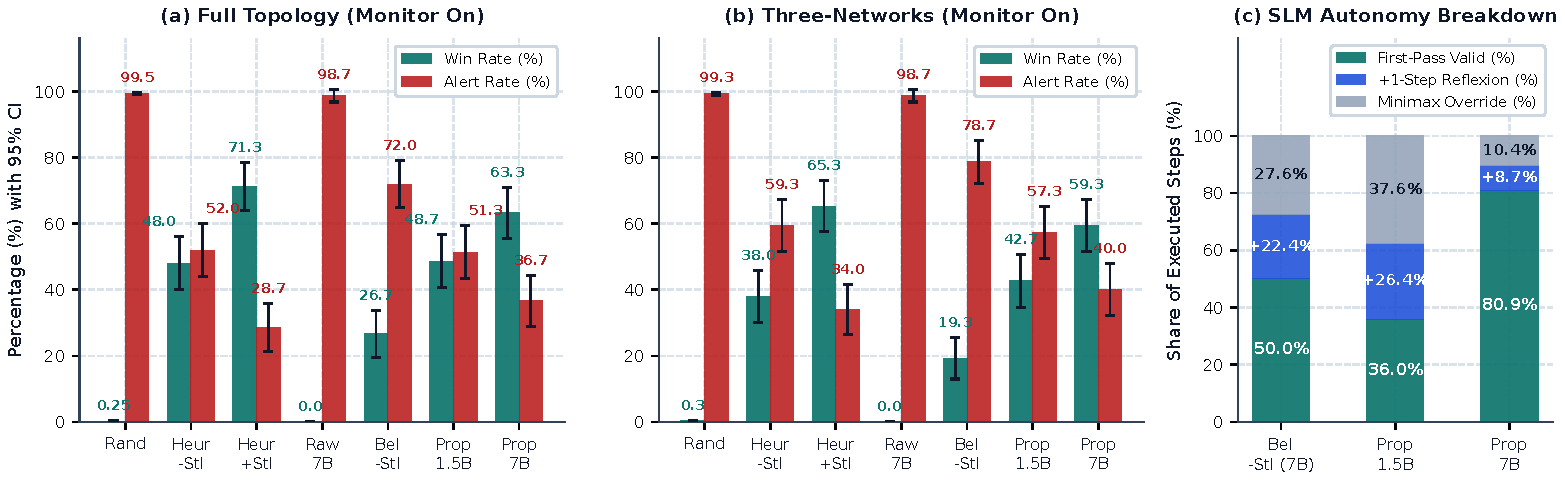
\includegraphics[width=0.92\textwidth]{figures/fig3_ablation_and_autonomy.pdf}
    \caption{(a)--(b) Win Rate (\%) and Monitor Alert Rate (\%) with 95\% confidence intervals across all 7 configurations ($n=150$ per agent; $n=2{,}000$ for \texttt{Random}) in \texttt{Full + Monitor On} and \texttt{Three-Networks + Monitor On}; (c) SLM Decision Autonomy Breakdown (\texttt{FirstPassValid~\%}, \texttt{+1-Step Reflexion Gain~\%}, and \texttt{Minimax Override~\%}).}
    \label{fig:ablation}
\end{figure*}

Table~\ref{tab:eswa_comparison} aligns our results directly with \citet{rigaki2026building} (Tables~4 and~5). Zero-shot \texttt{Proposed 7B-NF4} surpasses fine-tuned \texttt{Hackphyr-7B} across all four regimes via unpaired $z$-tests: \texttt{+9.57 pp} in \texttt{1A} ($z=+3.48, p=4.98 \times 10^{-4}$), \texttt{+19.33 pp} in \texttt{1B} ($z=+3.58, p=3.40 \times 10^{-4}$), \texttt{+44.33 pp} in \texttt{2A} ($z=+8.60, p=8.08 \times 10^{-18}$), and \textbf{\texttt{+36.00 pp} in \texttt{2B} (\texttt{59.33\%} vs.\ \texttt{23.33\%}, $z=+6.33, p=2.43 \times 10^{-10}$)}, while halving GPU memory from $\approx 14~\text{GB}$ to \texttt{5.91--5.92 GB}. It further outperforms cloud \texttt{GPT-4} on \texttt{Three-Networks NoDef} (\texttt{94.67\%} vs.\ \texttt{82.35\%}, $z=+2.36, p=0.0185$) and \texttt{Three-Networks + Monitor On} (\texttt{59.33\%} vs.\ \texttt{36.36\%}, $z=+2.31, p=0.0208$), flipping \texttt{GPT-4}'s \texttt{-21.69} return into \texttt{+12.08} under ESWA-50 parity (\texttt{+28.01} native) while matching \texttt{GPT-4} statistically in \texttt{Full} ($p \ge 0.304$). Even \texttt{1.5B-BF16} (\texttt{3.22 GB}) outperforms \texttt{Hackphyr-7B} in \texttt{1A} ($p=0.0408$), \texttt{2A} ($p=1.26 \times 10^{-11}$), and \texttt{2B} ($p=3.68 \times 10^{-4}$). Note that our \texttt{RandomAttacker} rate on \texttt{Full} (\texttt{4.65\%}) is lower than Table~4 of \citet{rigaki2026building} (\texttt{31.16\%}) because our YAML profiles randomize starting/goal hosts alongside \texttt{use\_dynamic\_addresses=True}.

\begin{table*}[t]
\centering
\caption{Direct comparison against exact published baselines from \citet{rigaki2026building} (Tables~4 and~5, \texttt{max\_steps = 100}). Cell format for our runs: \texttt{Win\% $\pm$ CI95 (Native / ESWA-50 Return)}. \texttt{Q-learning} required fixed episode IPs; all LLM/SLM runs use dynamic addressing.}
\label{tab:eswa_comparison}
\setlength{\tabcolsep}{3.0pt}
\footnotesize
\resizebox{\textwidth}{!}{%
\begin{tabular}{llcccc}
\toprule
Agent / Method & Peak VRAM / Compute & Full (NoDef) & Full (Mon. On) & Three-Nets (NoDef) & Three-Nets (Mon. On) \\
\midrule
\texttt{Random} (ESWA 2026 Ref) & CPU & $31.16 \pm 2.03$ ($-57.49$) & $2.72 \pm 0.71$ ($-66.56$) & $4.86 \pm 0.94$ ($-93.28$) & $0.13 \pm 0.16$ ($-70.73$) \\
\texttt{Random} (Ours, $n=2{,}000$) & CPU & $4.65 \pm 0.92$ ($-103.55 / -94.01$) & $0.25 \pm 0.22$ ($-32.24 / -71.99$) & $3.30 \pm 0.78$ ($-105.50 / -95.83$) & $0.30 \pm 0.24$ ($-32.29 / -71.97$) \\
\texttt{Q-learning} (ESWA 2026 Ref, fixed IPs) & CPU (50k ep train) & $67.71 \pm 4.09$ ($25.49$) & $\mathbf{71.57 \pm 3.95}$ ($42.94$) & $0.00 \pm 0.00$ ($-100.00$) & $0.00 \pm 0.00$ ($-70.45$) \\
\texttt{GPT-3.5-turbo} (ESWA 2026 Ref) & Cloud API & $30.00 \pm 16.40$ ($-51.67$) & $16.67 \pm 13.33$ ($-58.00$) & $10.00 \pm 10.73$ ($-87.50$) & $6.67 \pm 8.93$ ($-63.63$) \\
\texttt{Zephyr-7b-$\beta$} (ESWA 2026 Ref) & $\approx 14~\text{GB}$ FP16 & $23.65 \pm 4.80$ ($-51.77$) & $3.33 \pm 2.03$ ($-66.68$) & $1.75 \pm 1.97$ ($-98.80$) & $0.62 \pm 1.21$ ($-70.42$) \\
\texttt{Hackphyr} (ESWA 2026 Ref, SFT 7B) & $\approx 14~\text{GB}$ FP16 & $89.10 \pm 4.74$ ($61.03$) & $44.00 \pm 6.88$ ($3.56$) & $50.34 \pm 8.00$ ($-14.26$) & $23.33 \pm 6.77$ ($-37.67$) \\
\texttt{GPT-4} (ESWA 2026 Ref) & Cloud API & $\mathbf{100.00 \pm 0.00}$ ($77.13$) & $53.33 \pm 17.85$ ($8.80$) & $82.35 \pm 13.64$ ($18.78$) & $36.36 \pm 17.21$ ($-21.69$) \\
\midrule
\texttt{Proposed 1.5B-BF16} (Zero-Shot, Ours) & \textbf{3.22 GB} & $95.33 \pm 3.39$ ($+50.87 / +51.34$) & $48.67 \pm 8.03$ ($+16.01 / -4.53$) & $86.67 \pm 5.46$ ($+31.30 / +32.63$) & $42.67 \pm 7.94$ ($+8.48 / -14.45$) \\
\textbf{\texttt{Proposed 7B-NF4}} (Zero-Shot, Ours) & \textbf{5.91--5.92 GB} & $98.67 \pm 1.84$ ($+65.16 / +65.29$) & $63.33 \pm 7.74$ ($+36.11 / +21.45$) & $\mathbf{94.67 \pm 3.61}$ ($+52.05 / +52.58$) & $\mathbf{59.33 \pm 7.89}$ ($+28.01 / +12.08$) \\
\bottomrule
\end{tabular}%
}
\end{table*}

\subsection{Behavioral Mechanism, Entropy, and Architectural Takeaways}
Figure~\ref{fig:markov} explains these gains mechanically on \texttt{Three-Networks + Monitor On}: \texttt{RawReAct} traps itself in a \texttt{1.00} \texttt{ScanNetwork} self-loop ($H_t = 0.000$ bits); \texttt{NoStealth} exhibits \texttt{0.54} \texttt{FindServices}, \texttt{0.34} \texttt{ScanNetwork}, and \texttt{0.66} \texttt{ExfiltrateData} self-loops ($H_t = 0.968$ bits) that trip \texttt{GlobalDefender}; and \texttt{WithStealth} collapses self-loops to \texttt{0.04}, \texttt{0.11}, \texttt{0.02}, and \texttt{0.12} while channeling \texttt{FindServices} $\rightarrow$ \texttt{ExploitService} (\texttt{0.38}) and \texttt{ExploitService} $\rightarrow$ \texttt{FindData} (\texttt{0.70}), lifting entropy to $H_t = 1.774$ bits. Phase-arrival logs confirm earlier remote pivoting: \texttt{115/150} episodes reach \texttt{ExploitService} at median step \texttt{11.0} (mean \texttt{11.31}) under \texttt{WithStealth} in \texttt{2B}, versus \texttt{89/150} at median \texttt{14.0} (mean \texttt{14.63}) for \texttt{NoStealth} (and \texttt{111/150} at median \texttt{10.0} vs.\ \texttt{97/150} at \texttt{14.0} in \texttt{1B}). Figure~\ref{fig:pareto} shows sustained step-wise diversity ($H_t \approx 1.63$--$1.77$ bits) and strict Pareto dominance over \texttt{Hackphyr} and \texttt{GPT-4}.

\begin{figure*}[t]
    \centering
    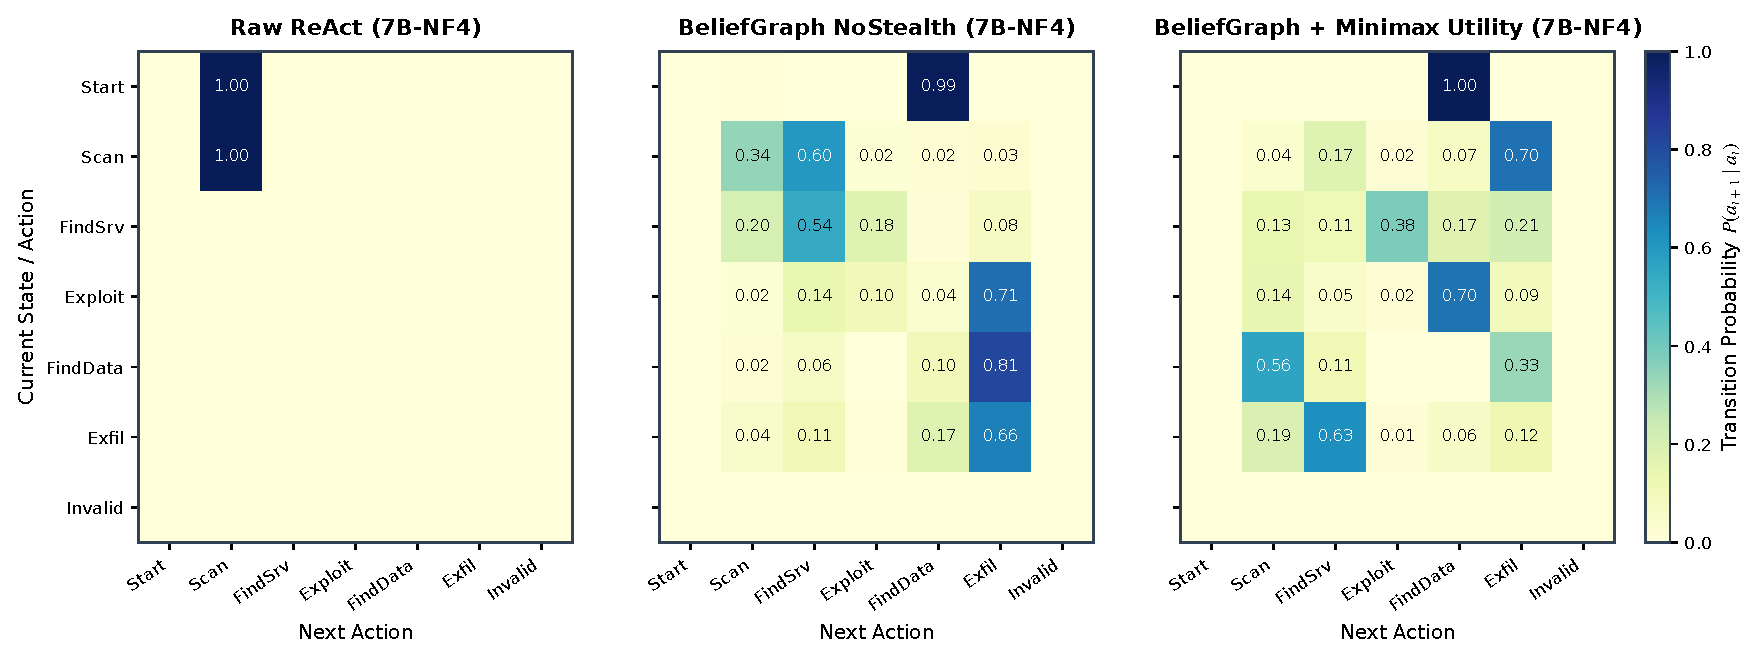
\includegraphics[width=0.92\textwidth]{figures/fig4_markov_transitions_comparison.pdf}
    \caption{Empirical 7$\times$7 Markov action-transition probability heatmaps in \texttt{Three-Networks + Monitor On} ($n=150$): (a) \texttt{RawReAct}, (b) \texttt{BeliefGraph\_NoStealth}, and (c) \texttt{Proposed BeliefGraph + Minimax Utility}.}
    \label{fig:markov}
\end{figure*}

\begin{figure*}[t]
    \centering
    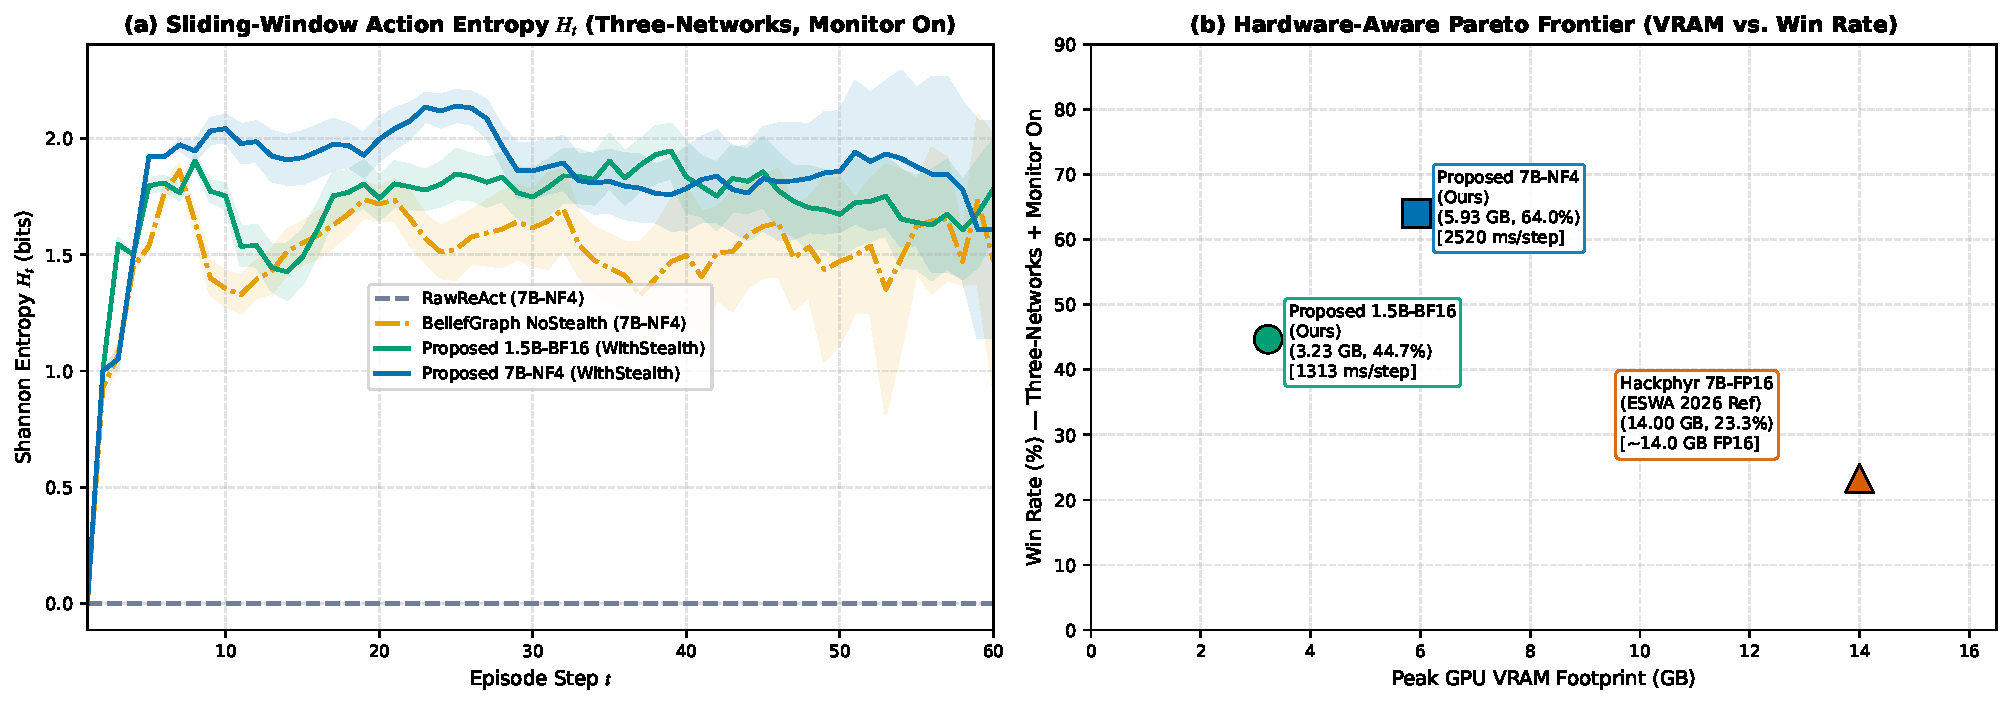
\includegraphics[width=0.92\textwidth]{figures/fig5_entropy_and_pareto.pdf}
    \caption{(a) Sliding-window Shannon action entropy $H_t$ ($w=5$, $t \le 60$ with 95\% CI shading) on \texttt{Three-Networks + Monitor On}, and (b) Hardware-Aware Pareto Frontier (peak GPU VRAM vs.\ Win Rate~\% and per-step latency) against ESWA 2026 \texttt{Hackphyr 7B-FP16} and \texttt{GPT-4}.}
    \label{fig:pareto}
\end{figure*}

\textbf{Why Architecture Beats Behavioral Cloning:} Static SFT on small undefended graphs locks \texttt{Hackphyr} into breadth-first enumeration habits that fail when \texttt{GlobalDefender} monitors multi-subnet expansion. Moreover, because \texttt{Qwen2.5-Coder-7B-NF4} scores \texttt{0.00\%} in \texttt{RawReAct} mode, base-model capability alone accounts for zero progress; decoupling $\mathcal{G}_t$ and $U(a)$ unlocks zero-shot generalization. Ranking candidates by $U(a)$ also lifts \texttt{7B-NF4} \texttt{FirstPass \%} autonomy from \texttt{45.53\%--50.84\%} (\texttt{NoStealth}) to \texttt{77.40\%--80.92\%}, and 1-step reflexion elevates \texttt{PostReflexion \%} to \texttt{85.76\%--89.63\%} (vs.\ \texttt{62.15\%--65.72\%} at \texttt{1.5B}, quantifying the sub-7B reasoning threshold).

\textbf{Limitations:} Three boundaries apply: (i) \texttt{10.37\%--14.24\%} of \texttt{7B-NF4} steps still invoke the $\arg\max_a U(a)$ fallback after two failed passes, motivating finite-state grammar decoding; (ii) \texttt{GlobalDefender} uses discrete window/streak rules, whereas production SOCs deploy ML detectors (\texttt{IsolationForest}, graph neural alerts); and (iii) evaluation covers single-attacker \texttt{NetSecGame} topologies.

\section{Conclusion and Future Work}
\label{sec:conclusion}

Directly addressing the open challenges in \citet{rigaki2026building}, this Research Note showed that pairing an untuned local SLM with a domain-agnostic Topological Belief Graph $\mathcal{G}_t$, Multi-Scale Minimax Hazard Utility $U(a)$ over $w \in \{3, 5, 8\}$, and 1-Step Counterfactual Reflexion with prefix KV-caching achieves \texttt{63.33\%} (\texttt{Full}) and \texttt{59.33\%} (\texttt{Three-Networks}) monitored win rates in under \texttt{5.92 GB} VRAM---outperforming fine-tuned \texttt{Hackphyr-7B} ($p \le 3.40 \times 10^{-4}$) and \texttt{GPT-4} ($p = 0.0208$ in \texttt{2B}) with zero task-specific training. Future work will generalize discrete window scales to continuous-time Hawkes exponential-decay hazard kernels with online Bayesian posterior estimation over $W^*$, integrate grammar-constrained logit masking to drive \texttt{Override~\%} toward zero, and test against adaptive ML blue-team defenders.

\printcredits

\section*{Declaration of competing interest}
The author declares that they have no known competing financial interests or personal relationships that could have appeared to influence the work reported in this paper.

\section*{Data availability}
{\sloppy Evaluation configurations, zero-hardcoding tests, consolidated summaries, statistical scripts, and plotting code are available at \url{https://github.com/AliTavakkoli80/NetSecGame} (branch \texttt{feature/stealth-belief-graph-slm}).\par}

\bibliographystyle{cas-model2-names}
\bibliography{references}

\end{document}
